\chapter{Reaction-Diffusion Systems}

	Reaction-diffusion (RD) systems are models that determine how concentrations of chemical species change in space. These systems are driven by two processes: chemical reaction and spatial diffusion. RD systems are governed by partial differential equations, the most basic of which might look something like
	\begin{align}
		\frac{\partial u}{\partial t} = d \nabla^2 u + r(u).
		\label{eq:KPP}
	\end{align}

This is sometimes called the Kolmogorov-Petrovsky-Piskounov equation in which $u$ is a generic chemical species, $d$ is a diffusion coefficient, $\nabla^2 u$ is the Laplace operator, and $r(u)$ is a general reaction term.	

RD systems are interesting because their solutions can show wide variety of patterns, many of which resemble patterns of nature such as spirals, stripes, and spots. In 1952, Alan Turing suggested that RD systems of morphogens, chemicals that govern the pattern of tissue development, may be able to explain the presence of spots or stripes on an organism\rf{turing_1952}. Although the science behind animal patterns is more complicated, Turing laid the framework by which patterns form from minor perturbations of otherwise homogenous systems. Since then, many others have noted the similarity between RD patterns and patterns in nature~\rf{bard_1974,bard_1981,murray_1981,meinhardt_1982,young_1984,turk_1991,witkin_1991}.
%\footnote{Among others, Bard, 1974 or 1981; Murray, 1981; Meinhardt, 1982; Young, 1984; Meinhardt and Klinger, 1987; or Turk, 1991.}

\begin{figure}[h]
	\centering
	\includegraphics[width=0.8\textwidth]{witkin}
         \caption{Patterns generated by reaction diffusion systems. Witkin compares these patterns to those of nature\rf{witkin_1991}; ``Row 1: reptile, giraffe, coral, scalloped. Row 2: spiral, triweave, twisty maze, replication, purple thing. Row 3: sand, maze, zebra haunch, radial. Row 4: space giraffe, zebra, stucco, beats us.'' Adapted from \protect\bibentry{witkin_1991}.} \label{fig:witkin}
\end{figure}
	
\section{The Gray-Scott Model} \label{sect:gsmodel}
	One important model in the study of pattern formation is the Gray-Scott system which models the reaction of two generic chemical species, $U$ and $V$\rf{grayscott_1984}. The model is based on the chemical reaction in \refeq{eq:gs-chem}.
	\begin{align}
	\begin{split}
		U + 2V &\rightarrow 3V \\
		V &\rightarrow P
		\label{eq:gs-chem}
	\end{split}
	\end{align}
$V$ is converted to inert product, $P$, which doesn't interfere with the reaction of the system. $V$ appears on both sides of the chemical reaction and thus catalyzes its own production. Gray and Scott developed the following non-dimensional PDE in which $u$ and $v$ represent the concentrations of chemicals $U$ and $V$ respectively.
	\begin{align}\label{eq:gs}
		\frac{\partial u}{\partial t} & = d_u \nabla^2 u - uv^2 + F(1-u) \\
		\frac{\partial v}{\partial t} & = d_v \nabla^2 v  + uv^2 - (F +k)v
	\end{align}
We see that both equations take the form of \refeq{eq:KPP} only they are coupled. For simplicity, $d_u$, $d_v$, $F$, and $k$ are taken to be constants. The first term in each equation, $d_u \nabla^2$ and $d_v \nabla^2$, are the diffusion terms. The Laplace operator, $\nabla^2$, is responsible for the diffusion of each chemical in space (like the diffusion of heat in the more familiar heat equation) while the \textit{diffusion coefficients}, $d_u$ and $d_v$, govern the diffusion rate. The $\pm uv^2$ terms are the  \textit{reaction terms} which convert $U$ into $V$: an increase in $v$ is equal to the decrease in $u$, hence $+uv^2$ in the second equation. Since $U$ will eventually get used up to generate $V$, the term $F(1-u)$ is the \textit{replenishment term} which reintroduces chemical $U$ into the system ($u$ has a maximum value of 1). Similarly, chemical $V$ would increase without limit except for the \textit{diminishment term}, $(F+k)v$, which serves to remove chemical $V$ from the system. $F$ is referred to the \textit{feed rate} and determines the rate of replenishment while $k$ is the difference between this rate and that of chemical $V$.

For some biological intuition, one can imagine the chemical reactions that occur in the development of an embryo as Turing theorized. In this case, the supply of chemicals might be the bloodstream where the replenishment and diminishment rates of the reaction are determined by the permeability of cell membranes.

The Gray-Scott system is particularly notable for the wide range of irregular patterns it produces. Previous analysis of the system by Pearson\rf{pearson_1993} identified at least 12 different pattern types, all of which occur at different $F, k$ with $d_u = 2 d_v$. \refFig{fig:pearson} shows the 12 quantifiably different patterns observed in this system determined by standard methods of nonlinear analysis\rf{strogatz_2001}. \refFig{fig:pearson_fk} shows provides a legend for the patterns, mapping each of them to their locations in $k, F$ parameter space. Each subfigure of \refFig{fig:pearson}, which plots the concentration of chemical $U$ over a 256 by 256 computational domain, reveal the extremely variable behavior of this system.\footnote{A concentration plot of $V$ would resemble the inverse of $U$ so only one is shown.} One of the most compelling qualities of these patterns is their resemblance to patterns of nature, \eg $\kappa$ (\refFig{fig:kappa_sample}) looks like coral and $\lambda$ (\refFig{fig:lambda_sample}) resembles the growth of bacteria. Other patterns, like $\beta$ (\refFig{fig:beta_sample}), exhibit turbulence.

\begin{figure}[h]
	\centering
	\begin{subfigure}[b]{0.2\textwidth}
                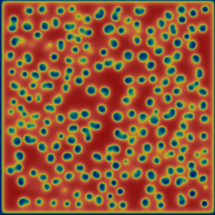
\includegraphics[width=\textwidth]{Figs/alpha_sample.png}
                \caption{$\alpha$}
                \label{fig:alpha_sample}
        \end{subfigure}%
        ~ %add desired spacing between images, e. g. ~, \quad, \qquad, \hfill etc.
          %(or a blank line to force the subfigure onto a new line)
        \begin{subfigure}[b]{0.2\textwidth}
                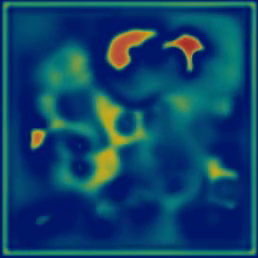
\includegraphics[width=\textwidth]{beta_sample.png}
                \caption{$\beta$}
                \label{fig:beta_sample}
        \end{subfigure}
        \begin{subfigure}[b]{0.2\textwidth}
                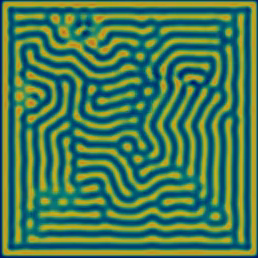
\includegraphics[width=\textwidth]{gamma_sample.png}
                \caption{$\gamma$}
                \label{fig:gamma_sample}
        \end{subfigure}
        \begin{subfigure}[b]{0.2\textwidth}
                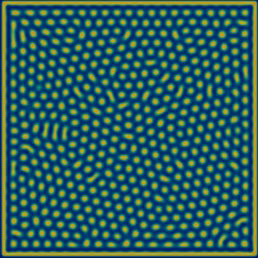
\includegraphics[width=\textwidth]{delta_sample.png}
                \caption{$\delta$}
                \label{fig:delta_sample}
        \end{subfigure} \hfill \\
         \begin{subfigure}[b]{0.2\textwidth}
                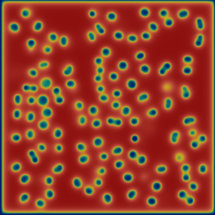
\includegraphics[width=\textwidth]{epsilon_sample.png}
                \caption{$\epsilon$}
                \label{fig:epsilon_sample}
        \end{subfigure}
        \begin{subfigure}[b]{0.2\textwidth}
                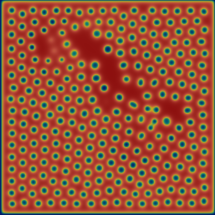
\includegraphics[width=\textwidth]{zeta_sample.png}
                \caption{$\zeta$}
                \label{fig:zeta_sample}
        \end{subfigure}
        \begin{subfigure}[b]{0.2\textwidth}
                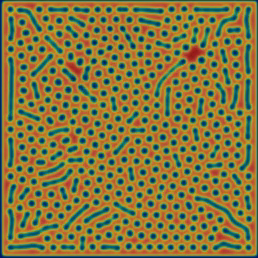
\includegraphics[width=\textwidth]{eta_sample.png}
                \caption{$\eta$}
                \label{fig:eta_sample}
        \end{subfigure}
        \begin{subfigure}[b]{0.2\textwidth}
                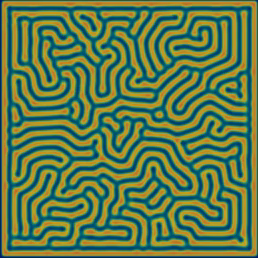
\includegraphics[width=\textwidth]{theta_sample.png}
                \caption{$\theta$}
                \label{fig:theta_sample}
        \end{subfigure} \hfill \\
        \begin{subfigure}[b]{0.2\textwidth}
                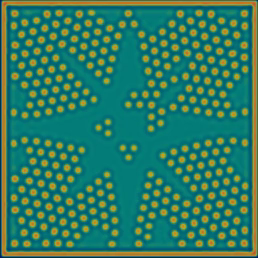
\includegraphics[width=\textwidth]{iota_sample.png}
                \caption{$\iota$}
                \label{fig:iota_sample}
        \end{subfigure}
         \begin{subfigure}[b]{0.2\textwidth}
                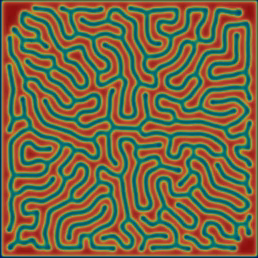
\includegraphics[width=\textwidth]{kappa_sample.png}
                \caption{$\kappa$}
                \label{fig:kappa_sample}
        \end{subfigure}
        \begin{subfigure}[b]{0.2\textwidth}
                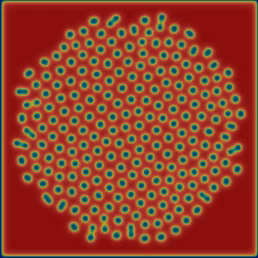
\includegraphics[width=\textwidth]{lambda_sample.png}
                \caption{$\lambda$}
                \label{fig:lambda_sample}
        \end{subfigure}
        \begin{subfigure}[b]{0.2\textwidth}
                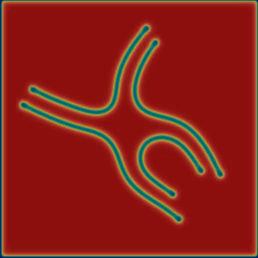
\includegraphics[width=\textwidth]{mu_sample.png}
                \caption{$\mu$}
                \label{fig:mu_sample}
        \end{subfigure} \hfill
        \caption{Patterns of chemical concentration $U$ identified in\rf{pearson_1993}. Each pattern, \refFig{fig:alpha_sample}---\refFig{fig:mu_sample}, is designated by a Greek letter which corresponds to the plot in \refFig{fig:fk_pspace}. Red and blue indicate $U=1$ and $U\approx 0.2$ respectively. Note that a concentration plot of chemical $V$ would appear as the inverse of $U$ with red and blue swapped.}\label{fig:pearson}
\end{figure}

\begin{figure}[h]
\begin{center}
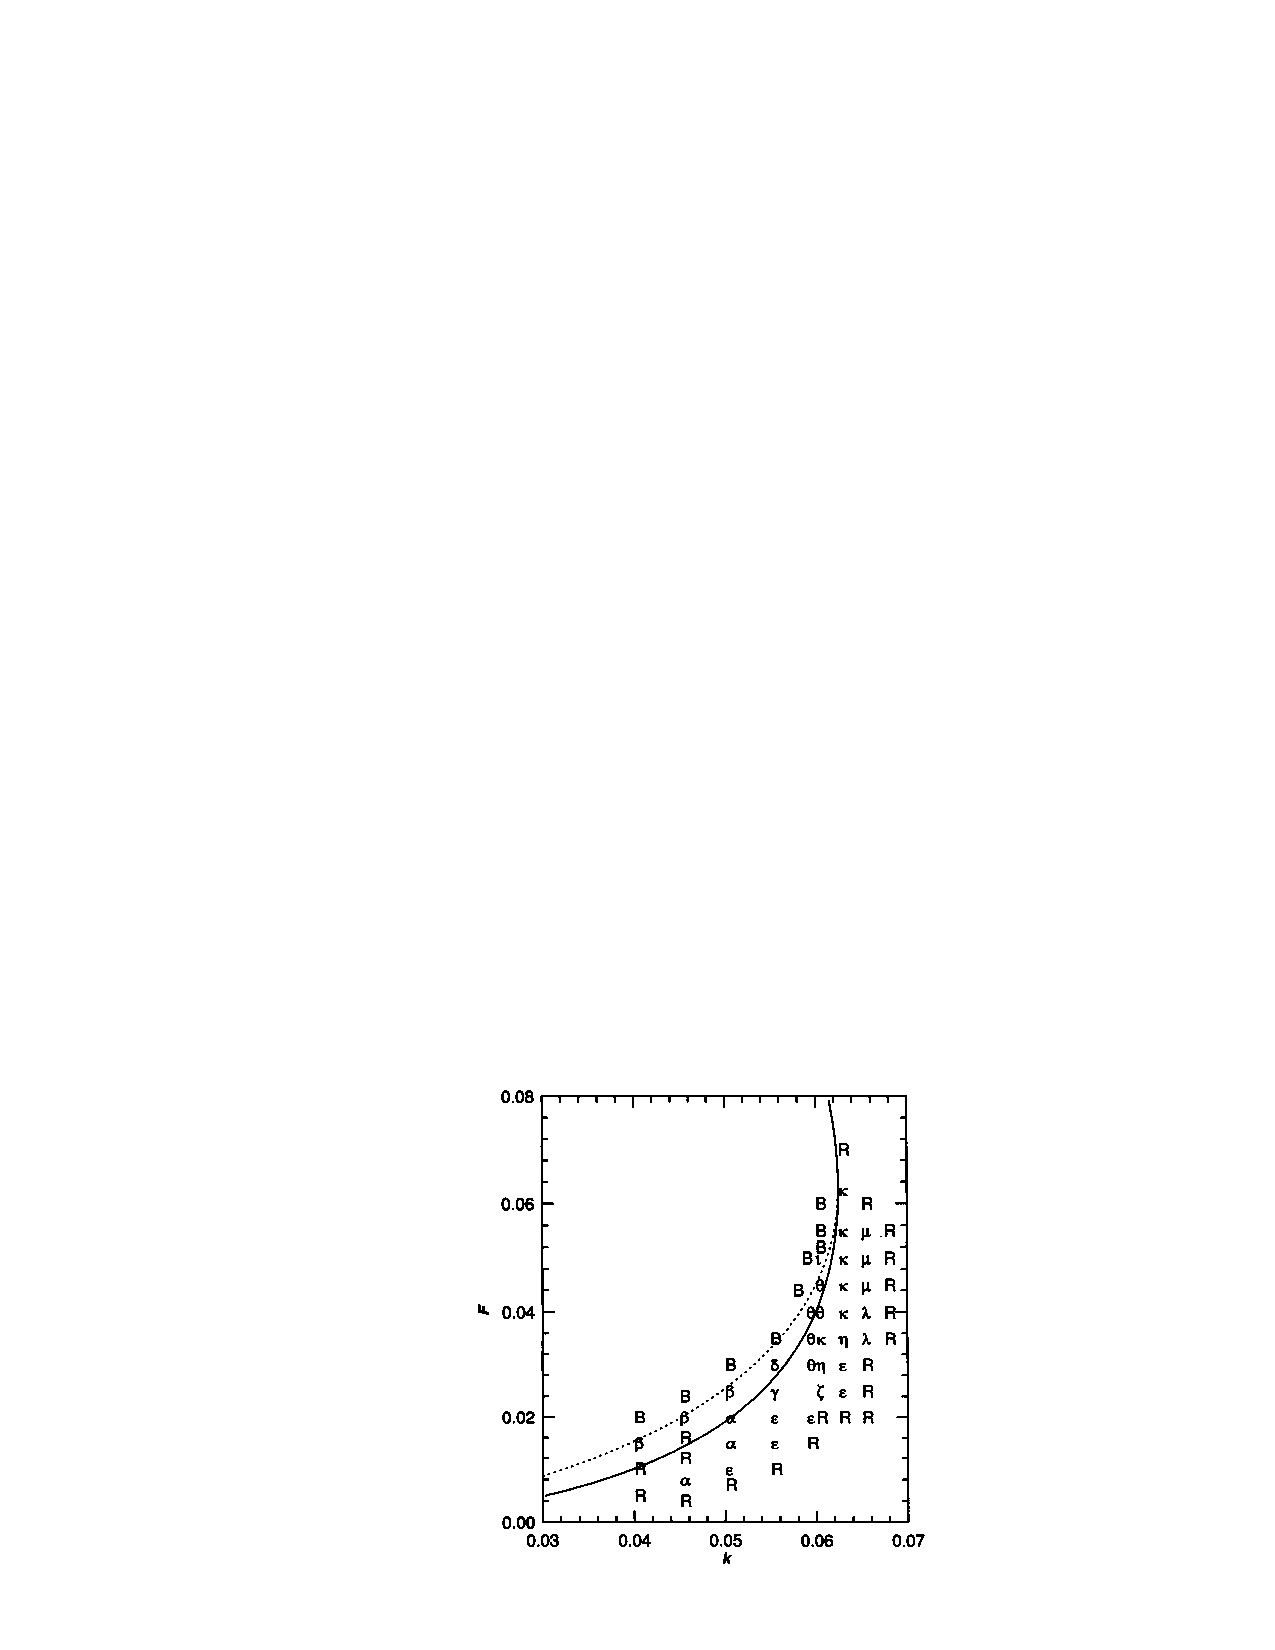
\includegraphics[width=0.5\columnwidth]{fk_pspace}
\caption{\label{fig:fk_pspace} The mapping of Greek letters in \refFig{fig:pearson} to their location in $k, F$ parameter space. R and B indicate that the system evolved to uniform red and blue states respectively. This figure also represents a phase diagram of the reaction kinetics. Between the solid and dotted line, the system is bistable for which there are two linearly stable steady states. As $f$ passes below the dotted line, the non-trivial steady state becomes unstable through Hopf bification giving stable periodic orbits for $k < 0.035$ and unstable for $k > 0.035$. The trivial state, ($U =1$, $V = 0$) exists for all $(f,k)$ outside the solid line. Adapted from \protect\bibentry{pearson_1993}.} \label{fig:pearson_fk}
\end{center}
\end{figure}

\section{Numerical Solution} \label{ch1:gs-simulation}

The system in \refeq{eq:gs} is solved by forward Euler integration of the discrete Laplacian obtained by the finite difference method shown in \refeq{eq:laplacian}.
	\begin{align}\label{eq:laplacian}
		\nabla^2 u(x,y) \approx u(x-1, y) + u(x+1, y) + u(x, y-1) + u(x, y+1) - 4 u(x, y)
	\end{align}
Similarly for $v$. In the Python programming language, this can be easily implemented using the Numpy package as below (see \refSect{appB:gs-code} for full code).
%
\begin{Verbatim}[fontsize=\footnotesize,frame=leftline,framesep=5mm]
Lu = ( U[0:-2,1:-1] + U[2: ,1:-1] + 
       U[1:-1,0:-2] + U[1:-1,2: ] - 4*U[1:-1,1:-1] )
Lv = ( V[0:-2,1:-1] + V[2: ,1:-1] + 
       V[1:-1,0:-2] + V[1:-1,2: ] - 4*V[1:-1,1:-1] )

uvv = u*v*v
u += (Du*Lu - uvv +  F   *(1-u))
v += (Dv*Lv + uvv - (F+k)*v    )
\end{Verbatim}

A spacial grid of $256 \times 256$ points constitutes the mesh with a time step of 1.\footnote{\rf{pearson_1993} notes no qualitative differences on mesh sizes up to $1024 \times 1024$ and time steps as low as $0.01$. Initial conditions also have little to no effect on the qualitative features of the resulting pattern after some time.} The system was initialized with the state $U=1$, $V=0$ with a $40 \times 40$ area located symmetrically in the center perturbed with $U=0.5$, $V=0.25$. This square area is then further sprinkled with 1\% random ``noise'' to catalyze the reaction. The patterns in \refFig{fig:pearson} were generated using this method and depict the concentration of chemical $U$. A plot of chemical $V$ would appear as the inverse. 

For each $F, k$, the simulation is run for 25,000 time steps. Every 10th image is saved, so a total of 2,500 PNG files are produced to describe the pattern. The pattern images that are analyzed by the methods described in \refChapter{ch:methods} use a greyscale colormap like that of \refFigs{fig:alphagrey}{fig:kappagrey}.



